\chapter{Венеция}
%\corner{64}
\vepsianrose

Погрузка заняла у них минут 40. Уклон местности выматывал с непривычки. Адмирал нацепил на ноги гидроноски на плотной подошве, и они с Замполитом спустили свои корабли на воду. Торжественный момент! Адмирал ждал его три года. Три года! Три года они не~ходили на~реку! У него чуть не~кружилась голова, хотя махнули лишь на~донышке. Он~снова на воде! Вот она, мокрая!!! Чистая!!! Карельская!!! Он~мечтал об этом очень, очень давно. И это свершалось\mdash сейчас, прямо на глазах.

В гидроносках шлёпать было гораздо удобнее, чем в~чём бы то ни было ещё\mdash можно было сразу с берега входить в воду и так же легко выходить, как босиком, не~боясь пораниться об камни, а толстая гидроткань защищала от~холода, напитываясь водой, которой передавалось тепло человеческого тела. Адмирал с Замполитом как раз рассекали в таких носках, защищавших их от прохладной карельской водички.

Замполит усердно распихивал гермы под борта своей байды. Адмирал, стоя в воде и ловя замполитову байду, отплывшую по инерции от очередного впихивания гермы, бросил тому:

\renewcommand*{\thefootnote}{\fnsymbol{footnote}}
%\renewcommand*{\thefootnote}{\arabic{footnote}}
\setcounter{footnote}{0}
\diagdash Кирь, привяжи байду за чалку\sdash то\footnote{Верёвка, трос для причаливания.}.

\diagdash У меня нету$\ldots$

\diagdash Да хар\'{о}ш! А чем чалиться собрался?!

Замполит пошёл искать чалку в вещах, а Адмирал, стоя по~колено в бодрящей водичке, стал принимать от~Руслана и Паши вещмешки и раскладывать их по~грузовому отсеку. Делать это стало труднее, чем обычно, потому что в~этот поход друзья прикупили байдарочные фартуки\mdash они уменьшили размеры погрузочного проёма. Адмирал, скрежетая зубами, раз за~разом пробовал по\sdash иному, компактнее впихивать снарягу. Лезло плохо, но он знал по~опыту\mdash всего через пару дней продуктов подуменьшится, и~всё будет влезать гораздо лучше.

\diagdash Давай фартук снимем, а наденем только перед порогами?\mdash предложил подошедший Замполит. 

\diagdash Умный, капец! А до порогов куда фартук денем? 

\diagdash На корму?

\diagdash У меня там спасжилеты, вот их точно только на~порогах наденем. Не, надо крепить фартуки, а то дождь собирается\mdash нальёт по~кильсон в трюмы!

\diagdash Ну, пожалуй$\ldots$

Серёга и Киря тоже, чертыхаясь, распихали всю снарягу под борта и по отсекам. У них была двушка, барахла влезло меньше. Начался дождь, повисла сплошная облачность, солнце не пробивалось. Адмирал, поморщившись, вытащил из кармана брезентовой штормовки дождевик, который всегда лежал у него в левом кармане штормовки, а~в~правом лежала кружка для отчерпывания воды и сугрева\mdash такова была привычка сплавщика. Команда тоже приоделась в~дождевики, кто во что.

\diagdash Готовы???

\diagdash ДА!

\diagdash Хрена два! Пойду проверю, что ничего не забыли!!!\mdash Адмирал пошёл наверх по склону к поляне, где собирали байды, чтобы самолично убедиться в отсутствии забытых вещей, и спустя пару минут, ничего не найдя, спустился обратно к~озеру, аккуратно ступая в~мокрых гидроносках:\mdash Ну, отчаливаем! Серёг, Паш, отвязывайте чалки!\mdash и~они с Замполитом заняли свои капитанские места\mdash в корме каждый своей байдарки. 

Поначалу только, неопытному байдарочнику, кажется это несправедливым\mdash мол, как же так, капитан и сидит на корме, где\sdash то на~галёрке. А все красоты реки первым усматривает сидящий впереди матрос. А ему, капитану, как бы всё позже доходит. Лишь спустя несколько речных переходов приходит понимание, что нет, всё правильно\mdash капитану с~кормы виднее всё на свете. Он лучше видит с кормы курс корабля, лучше усматривает куда сносит байдарку, как надо грести, чтобы обойти препятствия, как маневрировать. Да,~спины экипажа, конечно, закрывают вид прямо, но~это у Адмирала компенсировалось высоким ростом и~тем, что когда ходили по спокойным рекам, он, плевав на все правила, садился не~внутрь байдарки, а верхом на кормовой шпангоут. Таким образом, сидел он очень высоко, далеко видел, а насчёт устойчивости не~волновался\mdash матросы и вес груза в трюмах обеспечивали достаточный запас от~переворачиваемости. Сейчас же такой фокус не~прошёл\mdash сверху на фальшборта надели фартук, и~сидеть на кормовом шпангоуте стало невозможно\mdash тогда повредился бы~фартук. Адмиралу это было непривычно\mdash он за все свои предыдущие сплавы байдарочные свыкся с~мыслью, что всегда высоко сидит, далеко глядит, а~тут, как в первых сплавах, придётся сидеть низко\mdash хуже обзор воды. А~на~маршруте\mdash пороги. <<Ничего, справлюсь>>,\mdash подумал~он. В этот раз с ним был весь его предыдущий опыт, который, как известно, не пропьёшь. Он~с~силой оттолкнулся от~каменистого берега\mdash Cплав начался!

На небесах, тем временем, как кран открыли\mdash лило просто ужасно. У Руслана, который опрометчиво подумал, что, быть может, дождик скоро закончится, лёгкая курточка уже через 5 минут промокла насквозь, а кепку он и~вовсе никакую не взял\mdash плыл с непокрытой головой. Справа по~борту прошли торчащие изо дна озера жерди, на которых были растянуты то ли сети, то ли что\mdash похоже, тут~разводили рыбу. На берегу виднелся домик этого небольшого рыбохозяйства.

\diagdash Замполит, с Роман Менделичем, походу, договориться не~удалось, да?\mdash протирая ладонью капли дождя с носа, сказал Адмирал.

\diagdash Сам видишь, со связью тут швах, извиняй!\mdash отозвался тот с соседней байды.\mdash Но дождь уже задолбал, это точно!\mdash вид у~них в~дождевиках был так себе, почти комический. 

<<Пофиг, зато сухо>>,\mdash думал Адмирал. Руслан, отчего\sdash то не надевший дождевик, уже прилично так промок.

%\renewcommand*{\thefootnote}{\arabic{footnote}}
\renewcommand*{\thefootnote}{\fnsymbol{footnote}}
\setcounter{footnote}{0}
Бейдевинд\footnote{Бейдевинд (англ. by the wind)\mdash курс парусного судна относительно ветра, когда угол между диаметральной плоскостью судна и~направлением ветра составляет менее $90\degree$.} вперемешку с брызгами от вёсел экипажа выматывал. У западного конца Вендюрского озера Адмирал стал поглядывать в навигатор и прикидывать\mdash насколько велики шансы, что команда линчует его, если канал, по~которому он хотел сократить сегодняшний километраж примерно в полтора раза, попав в~речку Кулапдеги не~напрямую, а через Сяргозеро, окажется непроходим для байдарок. Минуты раздумья тянулись за~греблей томительно долго\mdash нетренированные мышцы рук, получившие убойный натиск от весла, ныли и не~давали сосредоточиться. Наконец, он решил\mdash была не была\mdash попробует ломиться через канал, интересно было глянуть что там.

К каналу подошли достаточно скоро и особо не искали его начало\mdash GPS был на контроле у Адмирала. Народ выразил ликование от такого сооружения, представшего их~взору. Канал был шириной примерно метров 8, а вот глубина оказалась крайне мала\mdash не более 20 сантиметров\mdash осадка байдарок еле\sdash еле позволяла проходить вперёд. Стенки канала были сделаны из брёвен, из воды показывалась пара венцов. Состояние брёвен Адмирал оценил максимум ещё лет на 10, неизвестно когда их обновляли в~последний~раз. Да~и~будут ли делать это снова\mdash кому это сейчас нужно$\quldots$ %?$\ldots$

\diagdash Саня! Там мель!\mdash увидал Паша. 

\diagdash Полундра, покинуть байду!\mdash скомандовал Адмирал, и далее по каналу они уже пошли шлёпая гидроносками по дну. Сверху было мокро от дождя, снизу от канала. <<Шикарное начало>>,\mdash подумал он, морщась.

\diagdash И мне вылазить?\mdash спросил Руслан. 

{
\setlength{\belowcaptionskip}{-5pt}
\begin{figure}[h]
	\centering
	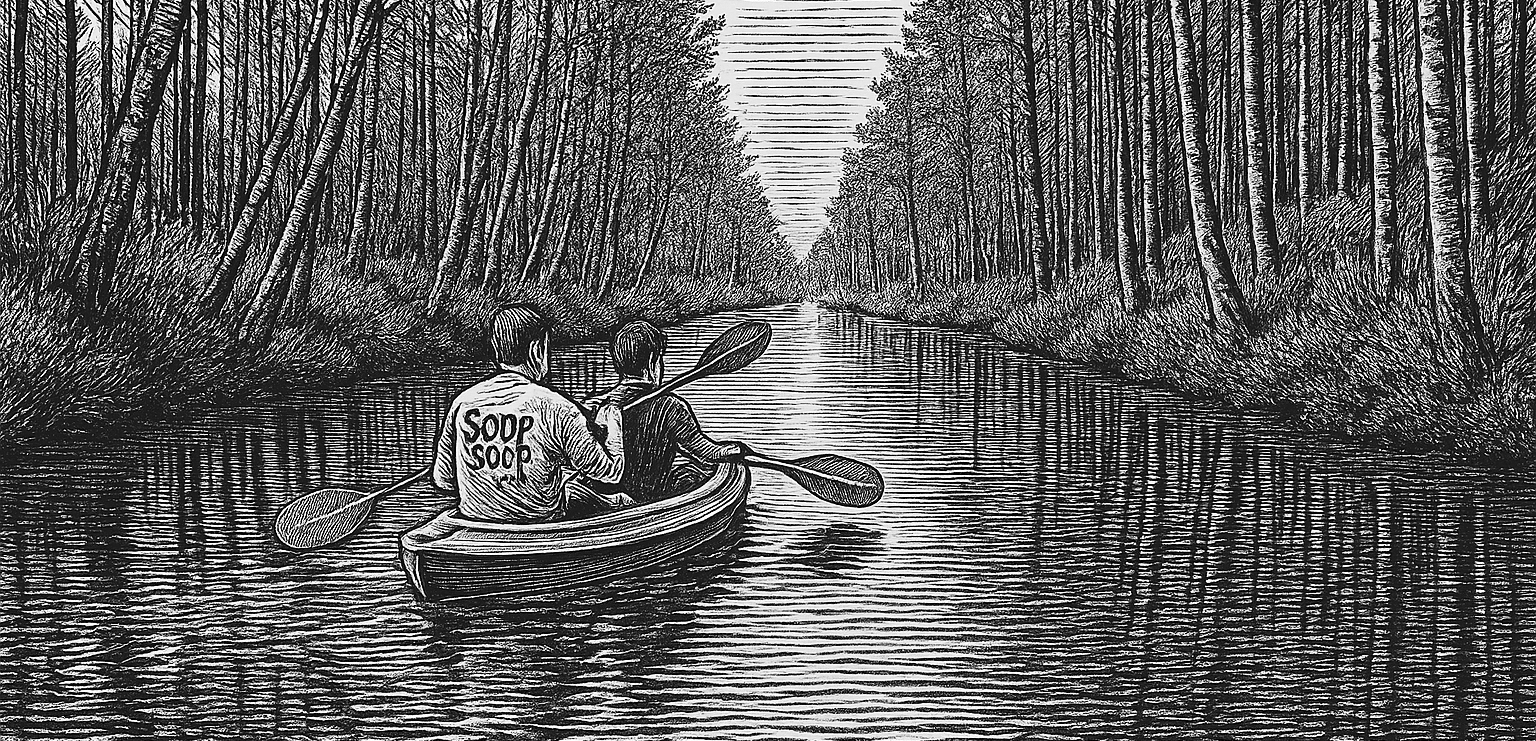
\includegraphics[width=1.0\textwidth]{14_channel}
	\caption{\small\textit{...Канал был шириной примерно метров 8...}}
\end{figure}

\diagdash Сиди, вроде осадка позволяет пока что!\mdash отозвался Адмирал, и они с Пашкой потихоньку стали проводить байду на чалке, стремясь не напороться на коряги и камни\mdash тот шёл спереди, подтаскивая байду за чалку, а Адмирал плёлся сзади, контролируя процесс.
%}

Вокруг канала были сплошные заросли, выглядела эта вся картина несколько сюрреалистично\mdash вдруг тут, в глуши, по какой\sdash то причине\mdash бах!\mdash и появился канал. Зачем появился, кто его сделал, с какой целью? Может рыбу разводили тут в советское время, а может и нет\mdash кто теперь расскажет? Ребята потихоньку продвигались вперёд то бредя по камням, то усаживаясь в байду, когда становилось чуть глубже. В~середине канала он стал совсем мелким, и им снова пришлось вылезти. Пеший переход по воде немного вымотал, надо было передохнуть. Через минут пять впереди показался конец канала, весь заросший тростником\mdash команда вышла в Сяргозеро. Решили устроить небольшой привал\mdash канал кончился, дождь выматывал, мышцы с непривычки ныли, а~Руслан промок до нитки.

\diagdash А ну, пацаны! Впереди стояночное место, что~ли?\mdash оценил Адмирал опытным взглядом небольшую бухту и~красивое место под соснами.

\diagdash Да вроде бы.\mdash отозвался Паша.

\diagdash Правим туда, перекур.\mdash скомандовал Адмирал. 

\diagdash Ура, ура, ура! Перекур!\mdash воскликнул Замполит, тоже порядком уже нагрёбшийся.

\diagdash Кирь, тебе <<привет>> от пульмонолога, какой перекур?\mdash язвил Шурик.

%\begin{figure}[h]
%	\centering
%	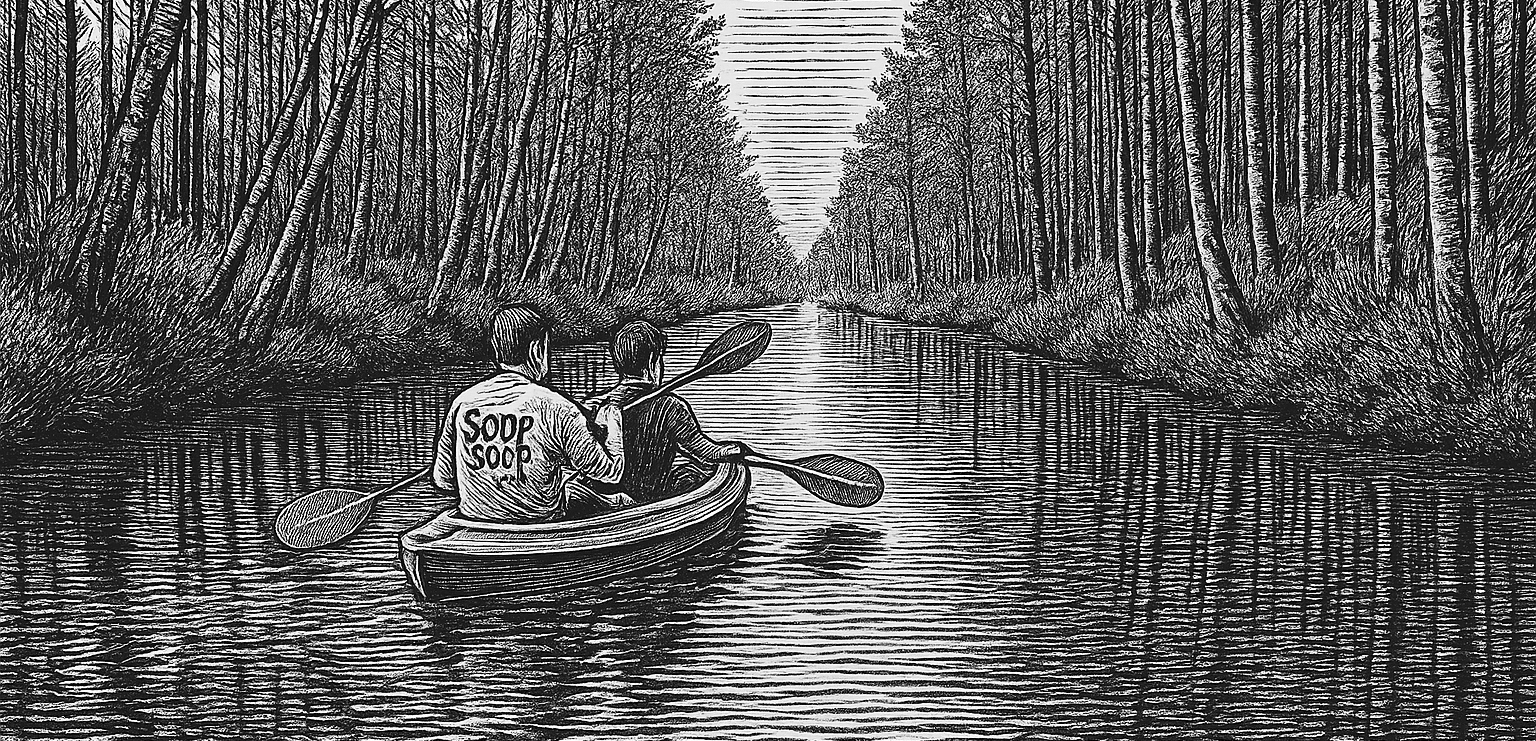
\includegraphics[width=1.0\textwidth]{7_gpt}
%	\caption{\small\textit{...Канал был шириной примерно метров 8...}}
%\end{figure}

\diagdash Шурик, иди-ка ты?

\diagdash Ы-ы-ы! Сигарку будешь?\mdash не унимался тот.

\diagdash Вы поглядите, вы поглядите! Совращают!

Естественно, едва оказавшись на берегу, Адмирал с~Замполитом смачно задымили. Серёга и Паша пошли осматривать стоянку, расположившуюся на левом берегу Сяргозера сразу после конца канала. Место было неоднозначным, но вполне себе подходящим под стоянку\mdash мусора почти не было, костровище имелось, полянка была хороша\mdash низкая трава и мшаник.

\diagdash Руслан, переодевайся, ты ж совсем промок!\mdash Адмиралу вдруг стало даже жалко своего новоиспечённого матроса. 

\diagdash Да блин, мою герму заложили мешками. Помоги?

\diagdash Давай, держу байду, доставай.\mdash Адмирал придержал байду, а Руслан вытащил шмот, переоделся, отжав куртку, и нацепил дождевик. 

Адмирал вернулся на берег\mdash осмотрел костровище, походил по поляне. Вокруг всё было, естественно, мокрым от дождя, который что\sdash то не собирался прекращаться. Теоретически, можно было бы остаться и~тут, за~километражом он решил абсолютно не~гнаться в~этом сплаве\mdash хватит, набегались за прошлые походы\mdash он решил почти что пустить это на самотёк, поскольку был уверен\mdash вторая часть маршрута по быстрой Суне с порогами будет скоростной$\ldots$ Только если, конечно, не~придётся ремонтировать байдарки после порогов. От дум Адмирала отвлёк Замполит:

\diagdash Твой матрос насквозь?

\diagdash Ага$\ldots$

\diagdash Бывает. Он первый раз в походе?

\diagdash Вроде как.

\diagdash Ладно, посмотрим как дальше пойдёт. Пора~вперёд\mdash греться веслом, чёт я замерзаю\mdash Замполит затушил окурок.

\diagdash Бригада! По коням!\mdash скомандовал Адмирал, и они стали отчаливать под дождём.

С двухкилометровым переходом через маленькое Сяргозеро Адмирал справился с трудом\mdash после передышки на~стоянке вообще не греблось, а встречный ветер выматывал. Но~он~не~имел права подать виду\mdash ведь он Адмирал сплава\mdash и грёб наравне со всеми. Замполит~же старательно упахивался веслом, предварительно закинувшись спортивным питанием, надеясь, как всегда, за~поход немного подкачаться. 

Думы вновь одолели Адмирала. Что если второй канал, по~которому он рассчитывал попасть из~Сяргозера в~реку Кулапдеги, зарос или обмелел, или и~то, и~то вместе взятое? А ещё хуже если завалило поперёк деревьями. Перспектива возвращаться назад в~Вендюрское озеро и~фактически начинать маршрут заново, с истока Кулапдеги, не то что не радовала, а просто уничтожала\mdash команда, во\sdash первых, такое не простит, и,~во\sdash вторых, это страшная и~бесполезная потеря времени и~сил. Адмирал решил положиться на удачу и в случае чего устроить волок\mdash перешеек между озером и рекой там всего 150\thinspace\nobreakdash---\thinspace 160~метров, он уже успел промерить по карте на перекуре. Но всё же перспективы он оценил верно\mdash если отметки урезов воды на~карте верны, то следующее озеро, как расположенное ниже по течению, должно было полноводнее, и воды в~канале будет достаточно для их байдарок. Команда медленно приближалась к~северной оконечности Сяргозера:

\diagdash Тащ Адмирал, разрешите обратиться?\mdash деланно язвил Замполит.\mdash А куда мы таки прёмся? Там озеро закончилось!

Тот поглядел на навигатор:

\diagdash Левее берём, нас относит боковым ветром. Канал должен быть левее!

\diagdash А если$\ldots$

\diagdash Никаких <<если>>! Канал левее!\mdash Адмирал что\sdash то мгновенно вспылил, отягощенный думами о канале и волоке.

\diagdash О, походу вон он!\mdash Серёга, Вперёдсмотрящий Кири, неопределённо показывал куда\sdash то вперёд.

Через 5 минут ребята без проблем прошли по~совсем короткому непримечательному полноводному каналу и~очутились в~речке Кулапдеги, уходящей влево дальше к Сяпчозеру. У~Адмирала отлегло\mdash первые два канала они миновали. Дальше начался в~буквальном смысле байдарочный слалом по петляющей среди сплошняковых болотистых лиственных зарослей речушке. По~прямой выходило километра три по карте, но~бесконечные повороты удлиняли путь чуть не в три раза:

\diagdash Шурик, это похоже на петляние Песи перед Хвойной.\mdash Замполит вдруг вспомнил былое.

\diagdash Ага, только болотина вокруг глянь какая! Ни~причалить, ни чего.

\diagdash Зато поворотики клёвые,\mdash отозвался Серёга.\mdash И~нет ветра, как на озере. Ищи плюсы!

\diagdash Эт да-а-а.\mdash согласился Адмирал. 

Ему речка эта, конечно, не понравилась. На стоянку в первый день, при планировании маршрута, он решил вставать уже на~Сяпчозере. Надо было просто, что называется, перетерпеть дождь и петляющую речку с~неприветливыми низкими болотистыми берегами. 

%\newpage
Адмирал погрузился в свои мысли. От~его взора на~карте не спрятался небольшой мыс по~правому берегу Сяпчозера. Он был расположен между двумя областями каменистого берега, обозначенного на старой топокарте. В~километре на северо\sdash восток оттуда располагался старый геодезический пункт на горе. Местность эта и этот мыс, расположенный между устьем Кулапдеги и истоком Сяпчи, понравились Адмиралу сразу. Сейчас он грёб, воплощая в~реальности своё перемещение в~пространстве к~стоянке. Он давно вывел для себя правило любого похода\mdash даже оказавшись на~маршруте впервые, ты обязан проходить его минимум в пятый раз! Первый\mdash читая описание маршрута в туристической литературе и~отчётах в Интернете, второй\mdash мысленно по~карте, топографической и спутниковой, третий\mdash в~разговорах и~обсуждениях с~товарищами, четвёртый\mdash мысленно соединяя, скрепляя воедино в~своем сознании предыдущие три раза и,~наконец, в~пятый раз уже в~реальности, на~местности. Район мыса между двух каменистых отмелей подходил под первую стоянку идеально\mdash они прошли порядка 14~километров в~первый день похода\mdash более чем достаточно. Адмирал также очень рассчитывал, что~относительная непопулярность этой части их маршрута оставит эту стоянку свободной\mdash первая стоянка должна подвести черту под началом их путешествия, преобразить вчерашних горожан в речных волков, очистить и перегрузить сознание всех и каждого\mdash он знал по опыту, что так всегда почему\sdash то случается, хотят сами сплавщики этого или нет. 

Небо наконец расчистилось, дождь кончился, как и~порядком надоевшая всем Кулапдеги, ребята оказались в~Сяпчозере. Переменчивая карельская погода, показав свой нрав, порадовала команду. Ласковое вечернее солнышко мгновенно подняло всем настроение, озёрный простор всем пришёлся по нраву после узкой петляющей речушки. Паша приободрился:

{
%\setlength{\belowcaptionskip}{-5mm}
\begin{figure}[h]
	\centering
	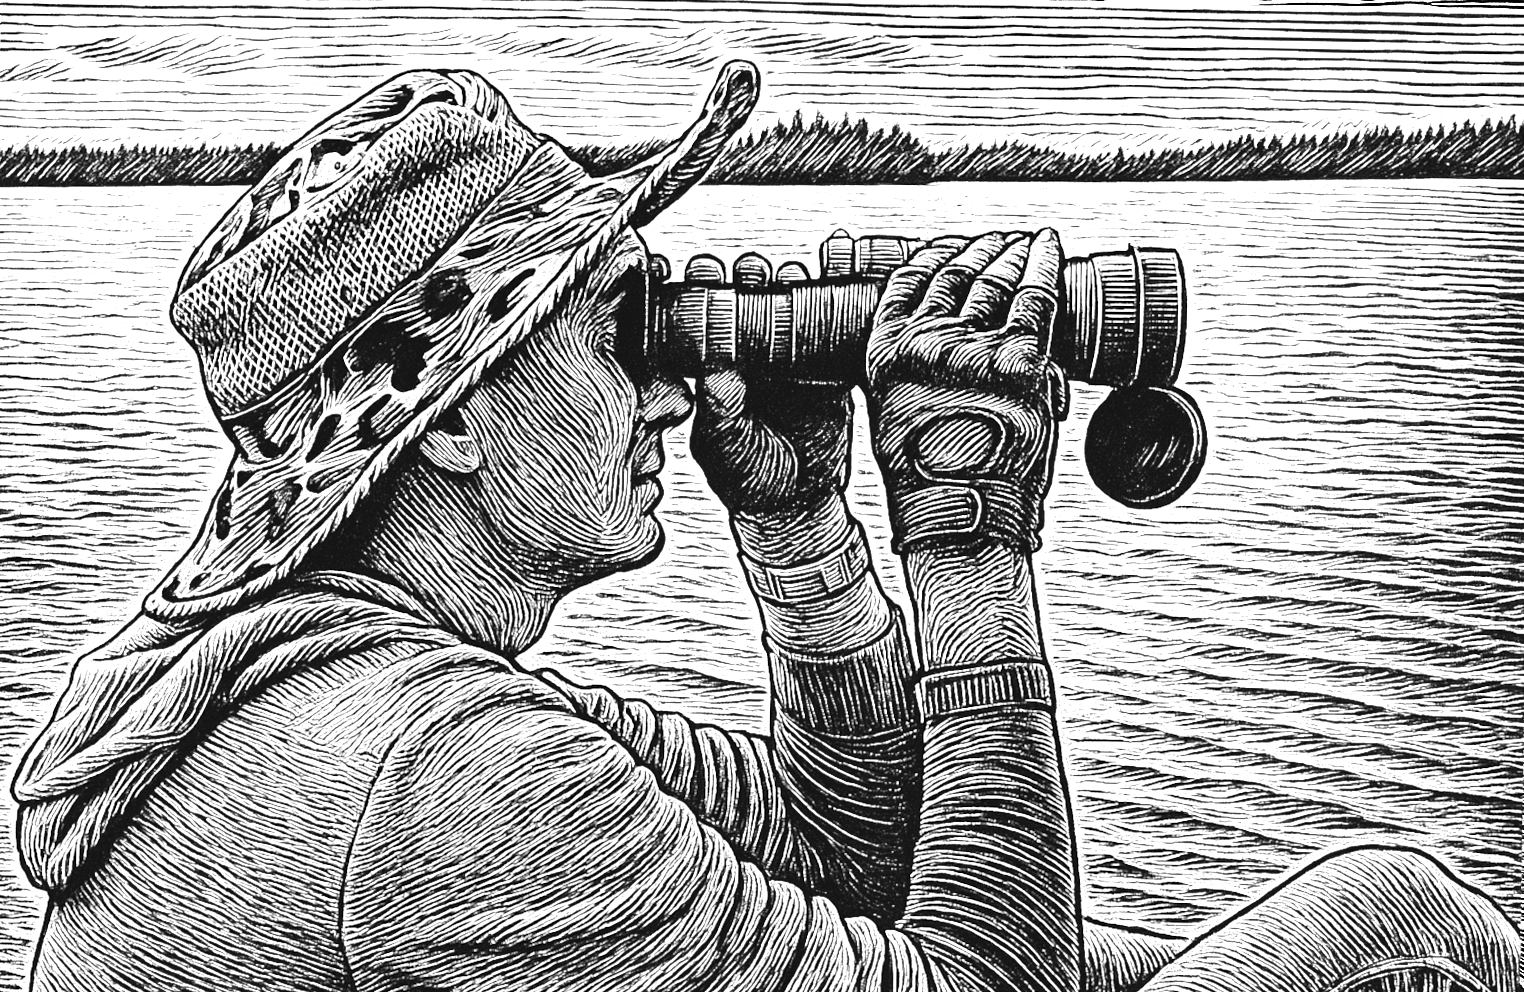
\includegraphics[width=1.0\textwidth]{15_1_okular}
	\caption{\small\textit{...ты говорил, что у тебя подзорная труба есть?..}}
\end{figure}

\diagdash Кирь, а ты говорил, что у тебя подзорная труба есть?
}

\diagdash Есть, ага! Специально взял стоянки искать по~озёрам.\mdash отозвался тот.  

\diagdash Щас самое время!

Они прошли начало каменистой отмели, оценив правый берег в её начале как малоперспективный в качестве стояночного. Киря достал трубу:

\diagdash Паш, на! У тебя зрение получше.

\diagdash Как тут чего?

\diagdash Крышки сними, окуляр крутится сзади.

\diagdash О! Туда!\mdash Пашка приник к трубе.\mdash Туда!!!

\diagdash Чё там?

\diagdash Мыс! Прямо по курсу!

<<Какая неожиданность>>,\mdash подумал Адмирал, радуясь, что команде тоже приглянулось <<его>> место.\mdash <<Конечно на~мыс, куда ж ещё>>.

Спустя совсем немного времени ребята оказались напротив мыса, где виднелась старая баня из полиэтиленовой плёнки. Место было хорошим\mdash высокие сосны, отсутствие кустарника наверху, снизу в воде\mdash камни. Типичная такая карельская стоянка, не чета верхневолжским. Выхода к воде со стоянки не было видно. 

\diagdash Шурик, где заберёмся?\mdash команде тоже не терпелось посмотреть стоянку, но берег был высоким\mdash едва можно было залезть с воды.

\diagdash Давай напролом к мысу, тут сто процентов где\sdash то должен быть хороший спуск к воде и проще его найти с~суши. Я~заберусь наверх и разведаю!\mdash они подошли к~юго\sdash западной оконечности мыса, и Адмирал вскарабкался на~небольшой обрыв, опираясь на весло.

\diagdash Ёклмн, вещи здесь таскать отстойно.\mdash начал Паша. 

%\setlength{\belowcaptionskip}{-5mm}
%\begin{figure}[h]
%	\centering
%	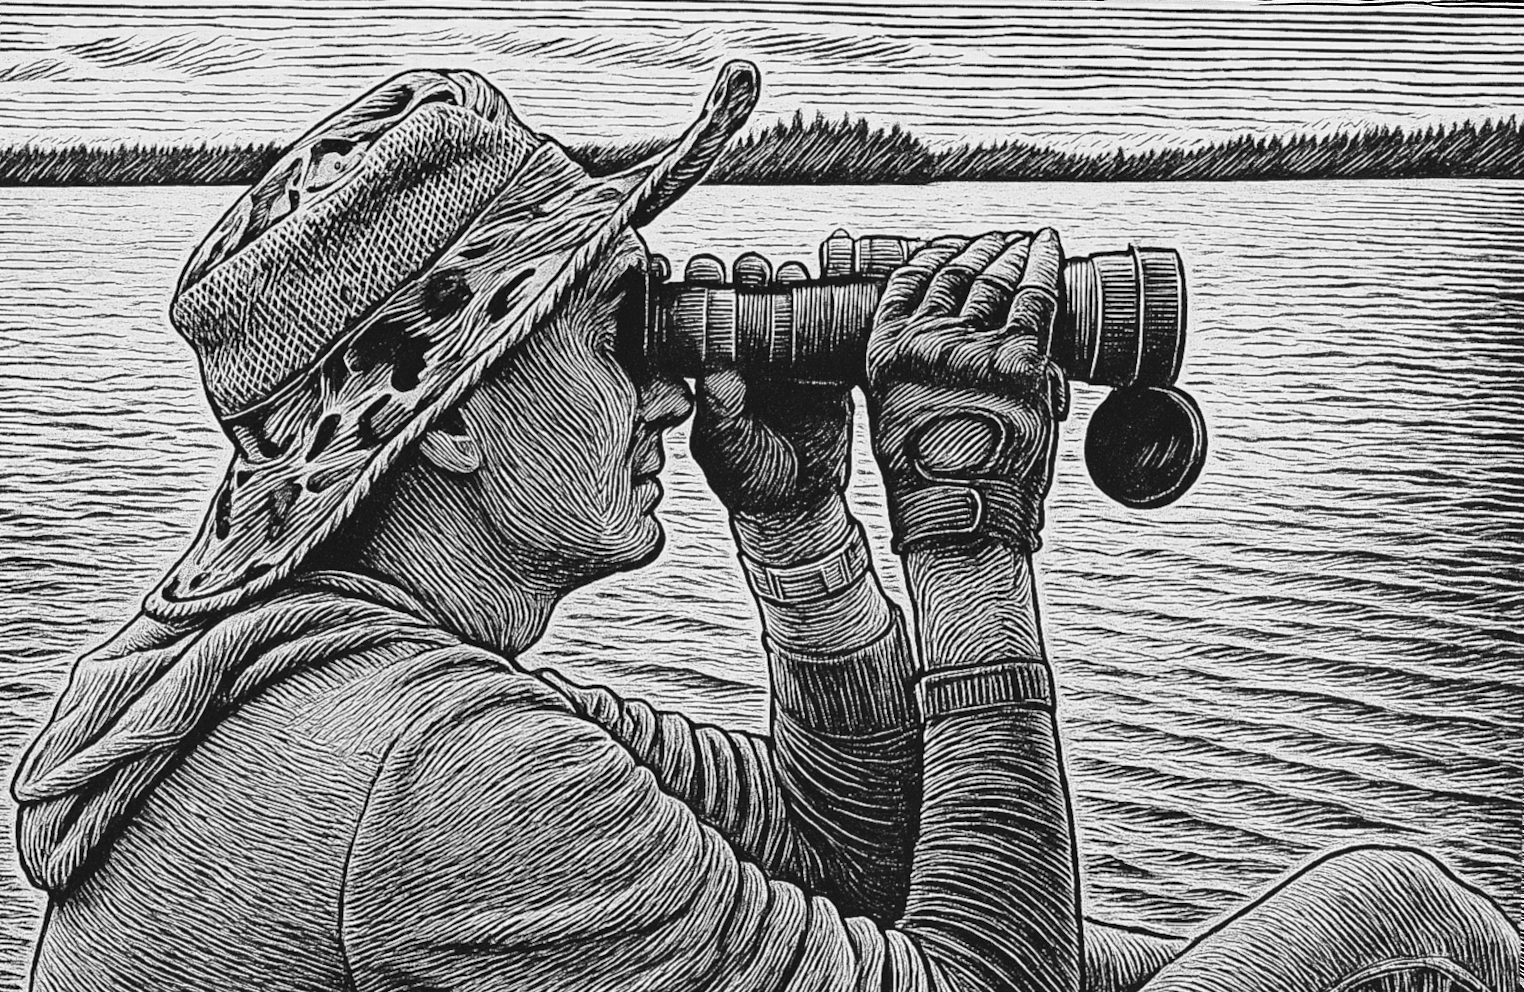
\includegraphics[width=1.0\textwidth]{7_gpt2}
%	\caption{\small\textit{...ты говорил, что у тебя подзорная труба есть?...}}
%\end{figure}

\diagdash Спокуха, я в разведку, а вы почильте тут пока.\mdash Адмирал быстро прошёлся по~мысу. Место было шикарным! В~глубине было местечко под пару палаток, в~наличии имелось старое костровище, остатки бани, скамейки из~брёвен. На самом мысу было ещё одно более менее ровное место под палатки, спуск к~воде уходил к~северной части мыса, обращённой к~берегу озера. Он разведал место для причаливания, и спустя ещё пару минут команда подвела туда свои корабли. Под две байдарки места не хватило, так что выгружались по очереди. Из~минусов стоянки, конечно, было то, что таскать вещи к костру\mdash далековато. Байдарки Адмирал велел далеко не тащить, а перевернуть для просушки тут же, в~паре метров от~<<причала>>.

Наконец, команда перетаскала вещи наверх, передохнули. Пока то да сё, Серёга и Паша успели забить места под палатки недалеко от костра, подальше от~воды вглубь мыса:

\diagdash Черти, а под адмиральскую палатку место?\mdash возмутился Шурик.

\diagdash Ну извиняй!

\diagdash На мысу комарья меньше будет!\mdash Замполит выбрал место под их с Адмиралом палатку на самом мысу, на второй ровной площадке.

\diagdash Я запо-о-омнил.\mdash медленно процедил Адмирал.

%\renewcommand*{\thefootnote}{\arabic{footnote}}
\renewcommand*{\thefootnote}{\fnsymbol{footnote}}
\setcounter{footnote}{0}
Команда быстренько натаскала дровишек, Адмирал собрал костровую перекладину из своих железных уголков и~подвесил над огнём шикарные овальные котелки, которые он приобрел на замену двум старым ещё в~2020\sdash м году на~выставке <<Рыболовство и~охота>>, как раз за пару месяцев до~всеобщего карантина по ковиду$\ldots$ Котелки ждали своего часа целых 3 года\mdash из нержавейки, удобные, с~крышками, складывающиеся <<матрёшкой>> друг в друга\mdash просто мечта походника. Хотя, по правде сказать, Адмирал мечтал о~титановых котелках, но цены на них были явно не~на~его нии\footnote{Научно-исследовательский институт.}\sdash шную зарплату$\ldots$

\vspace{0.01cm}
$\ldots$Спустя часа полтора у них уже почти всё было готово к~ужину. %Паша достал из мешка купленное у Олега в Гирвасе сало, а Замполит, сидя у костра в походном складном кресле, записывал видеозарисовки:
Замполит, сидя у костра в походном складном кресле, записывал видеозарисовки:

\diagdash Так, на костре у нас там суп и чай! А макароны$\ldots$ Уже сварены, остывают! Ой остывают, Шурик!

Паша немедленно подыграл:

\diagdash Хоп, у нас тут скромное меню, да. Мы~люди бедные, в~походе. Кочевники, можно сказать! Питаемся чем бог пошлёт, перебиваемся чем можем$\ldots$ Так,~чё~это? Убери,~я~нарежу сальца!\mdash он расчистил себе импровизированный столик, сооружённый из складного стульчика и фанерного байдарочного сиденья.

\diagdash А боги послали кусочек сала, Ы!\mdash Адмирал развалился во втором походном складном кресле в~предвкушении ужина.\mdash Ну, давайте, парни, подтягивайтесь, будем трапезничать!

Адмирал нарезал апельсин, достал, разлил: 

\diagdash Так, мужики, под горячее. Короче, без долгих речей. На маршрут встали\mdash молодцы, под дождём не скисли\mdash красавцы, два озера и два канала прошли\mdash ваще герои! Ну,~будем! Два отрывистых и одно раскатистое!!!

\diagdash {\large УРА, УРА, УРА\sdash А\sdash А!!!}\mdash грянула команда, послевкусие апельсинчика опосля тёмного выдержанного 7\sdash летнего рома было шикарным.

\diagdash Да, \textit{<<Венеция>>} была хороша сегодня.\mdash подытожил Серёга.\mdash Зачем только эти каналы прорыли?

\diagdash Мне тоже интересно, но, скорее всего, это надо бабушек да дедушек спрашивать, и то не факт, что знают. Это~ведь копали, я так думаю, уже более полувека назад.\mdash отозвался Адмирал.\mdash На наш век хватило увидеть, и это здорово, я никогда не бывал в таких местах.

\diagdash Я не первый раз в Карелии,\mdash Замполит нарезал ещё апельсина.\mdash но такого я тоже ещё не видал! Чтобы прям натуральный канал, брёвна и всё такое.%$\ldots$

%\vspace{0.2cm}
%$\ldots$
Команда отдыхала душой и телом. Место, на~котором Адмирал, согласно своему правилу, оказался в~пятый раз, хотя в реальности первый, было прекрасным. Настолько прекрасным, что как будто специально созданным всеми богами для туристической стоянки. Красота, полное отчуждение от цивилизации вместе с бравой командой, а~вокруг\mdash от природы дух захватывает! Высокие янтарные сосны, гладкие сереющие камни\sdash валуны, прибрежный зеленый камыш, оранжевое закатное солнце, окрашивающее всё вокруг в свои тёплые тона. Адмирал особенно любил начало августа, справедливо полагая это время года наиболее благоприятным для походов, сплавов их стиля. Он~даже временами мечтал, чтобы была в мире сила, способная сделать вечный август\mdash высокое звёздное небо, сбор урожая, тёплые деньки, не жаркое солнце. Словом,~среди всех времён года начало августа он любил больше~всего\mdash эти тёплые и мягкие деньки уносили его в~беззаботное детство, в деревню к родителям$\ldots$

\vspace{0.5cm}
$\ldots$Вокруг медленно спускалась ночь, но было ещё довольно светло\mdash характерная черта северных широт. На китайских ролексах Адмирала в окошечке даты стало появляться 1 августа. Мобильной связи не~было, как он и~хотел. Первый день прошёл как надо, он был доволен началом похода. Выключив ненавистные будильники на~6~утра в~телефоне, он с наслаждением понял, что завтра проснётся тогда, когда проснётся\mdash когда организм сам пожелает этого\mdash и~ни~одна дурацкая мысль о~будильнике и~необходимости вставать на~работу не~посмеет омрачить ему эту~неделю. 

\begin{center}
	\psvectorian[scale=0.4]{88} % Красивый вензелёк :)
\end{center}